% Asset ID: FA22LinearProgrammingFoundationsTikZ-002
% Source: Teacher transcript integer-solution discussion
% Purpose: nearby integer candidates around a non-integer optimum.
\documentclass[tikz,border=8pt]{standalone}
\usepackage{amsmath}
\usepackage{xcolor}
\usetikzlibrary{arrows.meta}
\definecolor{Canvas}{HTML}{FAF9F6}
\definecolor{Panel}{HTML}{FFFFF0}
\definecolor{LineSoft}{HTML}{E5E5EA}
\definecolor{Accent}{HTML}{C5A059}
\definecolor{Gold}{HTML}{D4AF37}
\definecolor{SoftPink}{HTML}{FBEFEF}
\definecolor{Text}{HTML}{2C2C2E}
\begin{document}
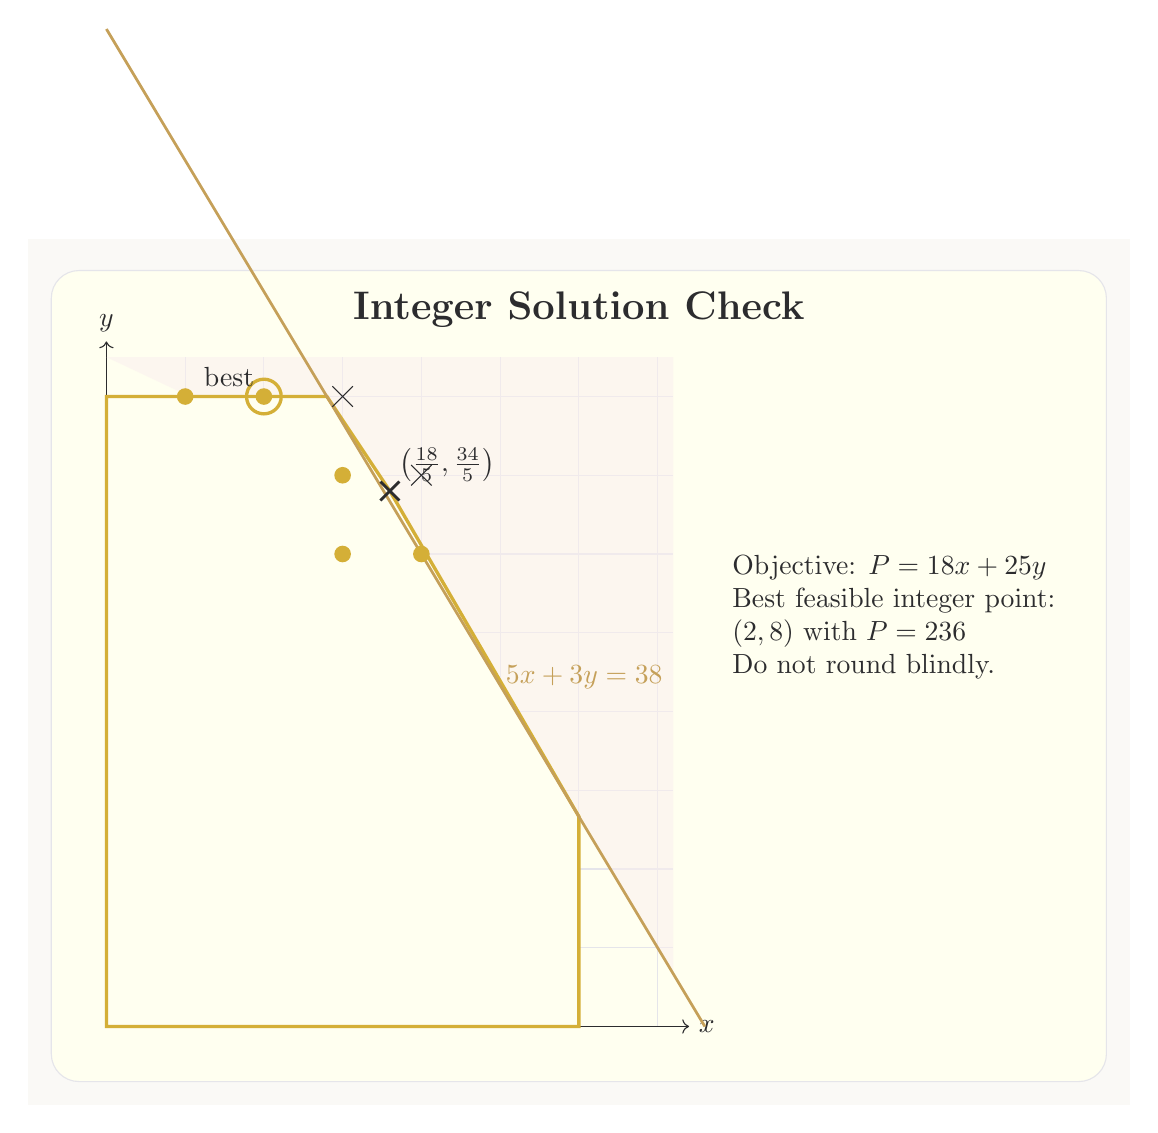
\begin{tikzpicture}[x=1cm,y=1cm]
\fill[Canvas] (-1,-1) rectangle (13,10);
\fill[Panel,rounded corners=10pt,draw=LineSoft] (-.7,-.7) rectangle (12.7,9.6);
\node[Text,font=\Large\bfseries] at (6,9.1) {Integer Solution Check};
\foreach \x in {0,...,7}{\draw[LineSoft] (\x,0)--(\x,8.5);}
\foreach \y in {0,...,8}{\draw[LineSoft] (0,\y)--(7.2,\y);}
\draw[Text,->] (0,0)--(7.4,0) node[right] {$x$};
\draw[Text,->] (0,0)--(0,8.7) node[above] {$y$};
\fill[SoftPink,opacity=.5] (0,8.5)--(7.2,8.5)--(7.2,.67)--(3.6,6.8)--cycle;
\fill[Panel] (0,0)--(0,8)--(2.8,8)--(3.6,6.8)--(6,2.667)--(6,0)--cycle;
\draw[Gold,line width=1.2pt] (0,0)--(0,8)--(2.8,8)--(3.6,6.8)--(6,2.667)--(6,0)--cycle;
\draw[Accent,line width=1pt] (0,12.667)--(7.6,0) node[pos=.65,right] {$5x+3y=38$};
\draw[Text,line width=1pt] (3.48,6.68)--(3.72,6.92);\draw[Text,line width=1pt] (3.48,6.92)--(3.72,6.68);
\node[Text,above right] at (3.6,6.8) {$\left(\frac{18}{5},\frac{34}{5}\right)$};
\foreach \x/\y in {3/6,3/7,4/6,2/8,1/8}{\fill[Gold] (\x,\y) circle (3pt);}
\draw[Gold,line width=1.2pt] (2,8) circle (.22);
\node[Text,above left] at (2,8) {best};
\foreach \x/\y in {4/7,3/8}{\draw[Text] (\x-.13,\y-.13)--(\x+.13,\y+.13);\draw[Text] (\x-.13,\y+.13)--(\x+.13,\y-.13);}
\node[Text,align=left] at (10,5.2) {Objective: $P=18x+25y$\\Best feasible integer point:\\$(2,8)$ with $P=236$\\Do not round blindly.};
\end{tikzpicture}
\end{document}
